%%  Chapter 3 - Data and Methodology

\ifpdf
\graphicspath{{chapters/Figs/}{chapters/Figs/Raster/}{Figs/PDF/}{Figs/}}
\else
\graphicspath{{chapters/Figs/}{chapters/Figs/Vector/}{Figs/}}
\fi

\chapter{Data and Methodology}
\label{ch:methodology}

\section{Data Sources}
\label{sec:data_sources}

\subsection{ERA5 Reanalysis}
\label{subsec:era5}

The primary dataset is the ERA5 global reanalysis produced by the
European center for Medium-Range Weather Forecasts (ECMWF)
\autocite{hersbach2020era5}. ERA5 provides hourly estimates of
atmospheric, land-surface, and oceanic variables on a regular
latitude-longitude grid at $0.25^\circ \times 0.25^\circ$ horizontal
resolution (approximately 28\,km at the equator), with 37 pressure
levels from 1000\,hPa to 1\,hPa. The dataset is generated through a
4D-Var data assimilation system that ingests conventional and
satellite observations \autocite{hersbach2020era5}.

The following ERA5 surface and single-level fields are used at hourly
temporal resolution over the domain 5-35$^\circ$N, 60-100$^\circ$E:

\begin{itemize}
  \item \textbf{850\,hPa relative vorticity} (\texttt{vo}): MD
    detection, tracking, and center identification.
  \item \textbf{Mean sea-level pressure} (\texttt{msl}):
    closed-circulation verification.
  \item \textbf{Surface latent heat flux} (\texttt{slhf},
    J\,m$^{-2}$, accumulated): de-accumulated to W\,m$^{-2}$;
    positive upward throughout.
  \item \textbf{Surface sensible heat flux} (\texttt{sshf},
    J\,m$^{-2}$, accumulated): de-accumulated identically.
  \item \textbf{Volumetric soil water layer\,1} (\texttt{swvl1},
    m$^3$\,m$^{-3}$): 0-7\,cm near-surface soil moisture, instantaneous.
  \item \textbf{Total precipitation} (\texttt{tp}, m\,hr$^{-1}$,
    accumulated): de-accumulated to mm\,hr$^{-1}$.
  \item \textbf{2-m dewpoint temperature} (\texttt{d2m}, K):
    boundary-layer moisture saturation state.
  \item \textbf{2-m temperature} (\texttt{t2m}, K): surface thermodynamic state.
  \item \textbf{Land-sea mask} (\texttt{lsm}): land/ocean
    classification (\texttt{lsm} $\geq 0.5$ = land).
  \item \textbf{10-m U and V wind components} (\texttt{u} and
    \texttt{v}, ms$^{-1}$): translational flow environment.
\end{itemize}

ERA5 accumulated flux variables are de-accumulated to instantaneous values as:
\begin{equation}
  F_\mathrm{inst}(t) = \frac{F_\mathrm{acc}(t) - F_\mathrm{acc}(t -
  1\,\mathrm{h})}{\Delta t_s},
  \label{eq:deaccumulate}
\end{equation}
where $F_\mathrm{acc}$ is the accumulated value in J\,m$^{-2}$ and
$\Delta t_s = 3600$\,s. ERA5 uses a sign convention in which LHF is
negative upward; this convention is corrected throughout so that
positive values denote upward flux.

\begin{table}[h]
  \centering
  \caption[Summary of ERA5 variables]{ERA5 variables, identifiers,
  processed units, analysis roles.}
  \label{tab:variables_summary}
  \begin{tabular}{l l l l}
    \toprule
    \textbf{Variable} & \textbf{ERA5 ID} & \textbf{Units} & \textbf{Role} \\
    \midrule
    850\,hPa relative vorticity & \texttt{vo}     &
    $10^{-5}$\,s$^{-1}$  & MD detection \\
    Mean sea-level pressure      & \texttt{msl}    & hPa
    & Circulation check \\
    Surface latent heat flux     & \texttt{slhf}   & W\,m$^{-2}$
    & BOE indicator \\
    Surface sensible heat flux   & \texttt{sshf}   & W\,m$^{-2}$
    & Energy partitioning \\
    Soil water (0-7\,cm)        & \texttt{swvl1}  & m$^3$\,m$^{-3}$
    & BOE, \\
    Total precipitation          & \texttt{tp}     & mm\,hr$^{-1}$
    & Feedback, Hovmöller \\
    2-m dewpoint temperature     & \texttt{d2m}    & K
    & BL moisture \\
    2-m temperature              & \texttt{t2m}    & K
    & Bowen ratio \\
    Land-sea mask                & \texttt{lsm}    & fraction
    & Phase classification \\
    \bottomrule
  \end{tabular}
\end{table}

\subsection{SRTM Elevation Data}
\label{subsec:srtm}

Shuttle Radar Topography Mission (SRTM) 1-arc-second ($\approx
30$\,m) DEM tiles in HGT format are used for terrain
characterization. Tiles are loaded and interpolated to track
positions by bilinear interpolation.

\subsection{IMD Monsoon Seasonal Reports}
\label{subsec:imd_data}

The India Meteorological Department (IMD) publishes annual Monsoon
Seasonal Reports providing synoptic track information for all LPS
over the north Indian Ocean, including formation date, landfall time,
landfall location, and dissipation time. These reports are used to
cross-validate ERA5-derived MD tracks.

\section{Study Domain and Period}
\label{sec:domain}

% FULL_EXTENT = [70.0, 95.0, 7.0, 30.0]  # lon_min, lon_max, lat_min, lat_max
The analysis covers June-September for 2001-2025. The ERA5 extraction
domain (over Indian subcontinent and surrounding ocean) is
7-30$^\circ$N, 70-95$^\circ$E shown in Figure~\ref{fig:study_domain}.

%%  FIGURE: Study domain map
%%  Show ERA5 domain box, detection domain box (inner), Eastern Ghats
% contours, BoB, and preferred landfall zone
\begin{figure}[H]
  \centering
  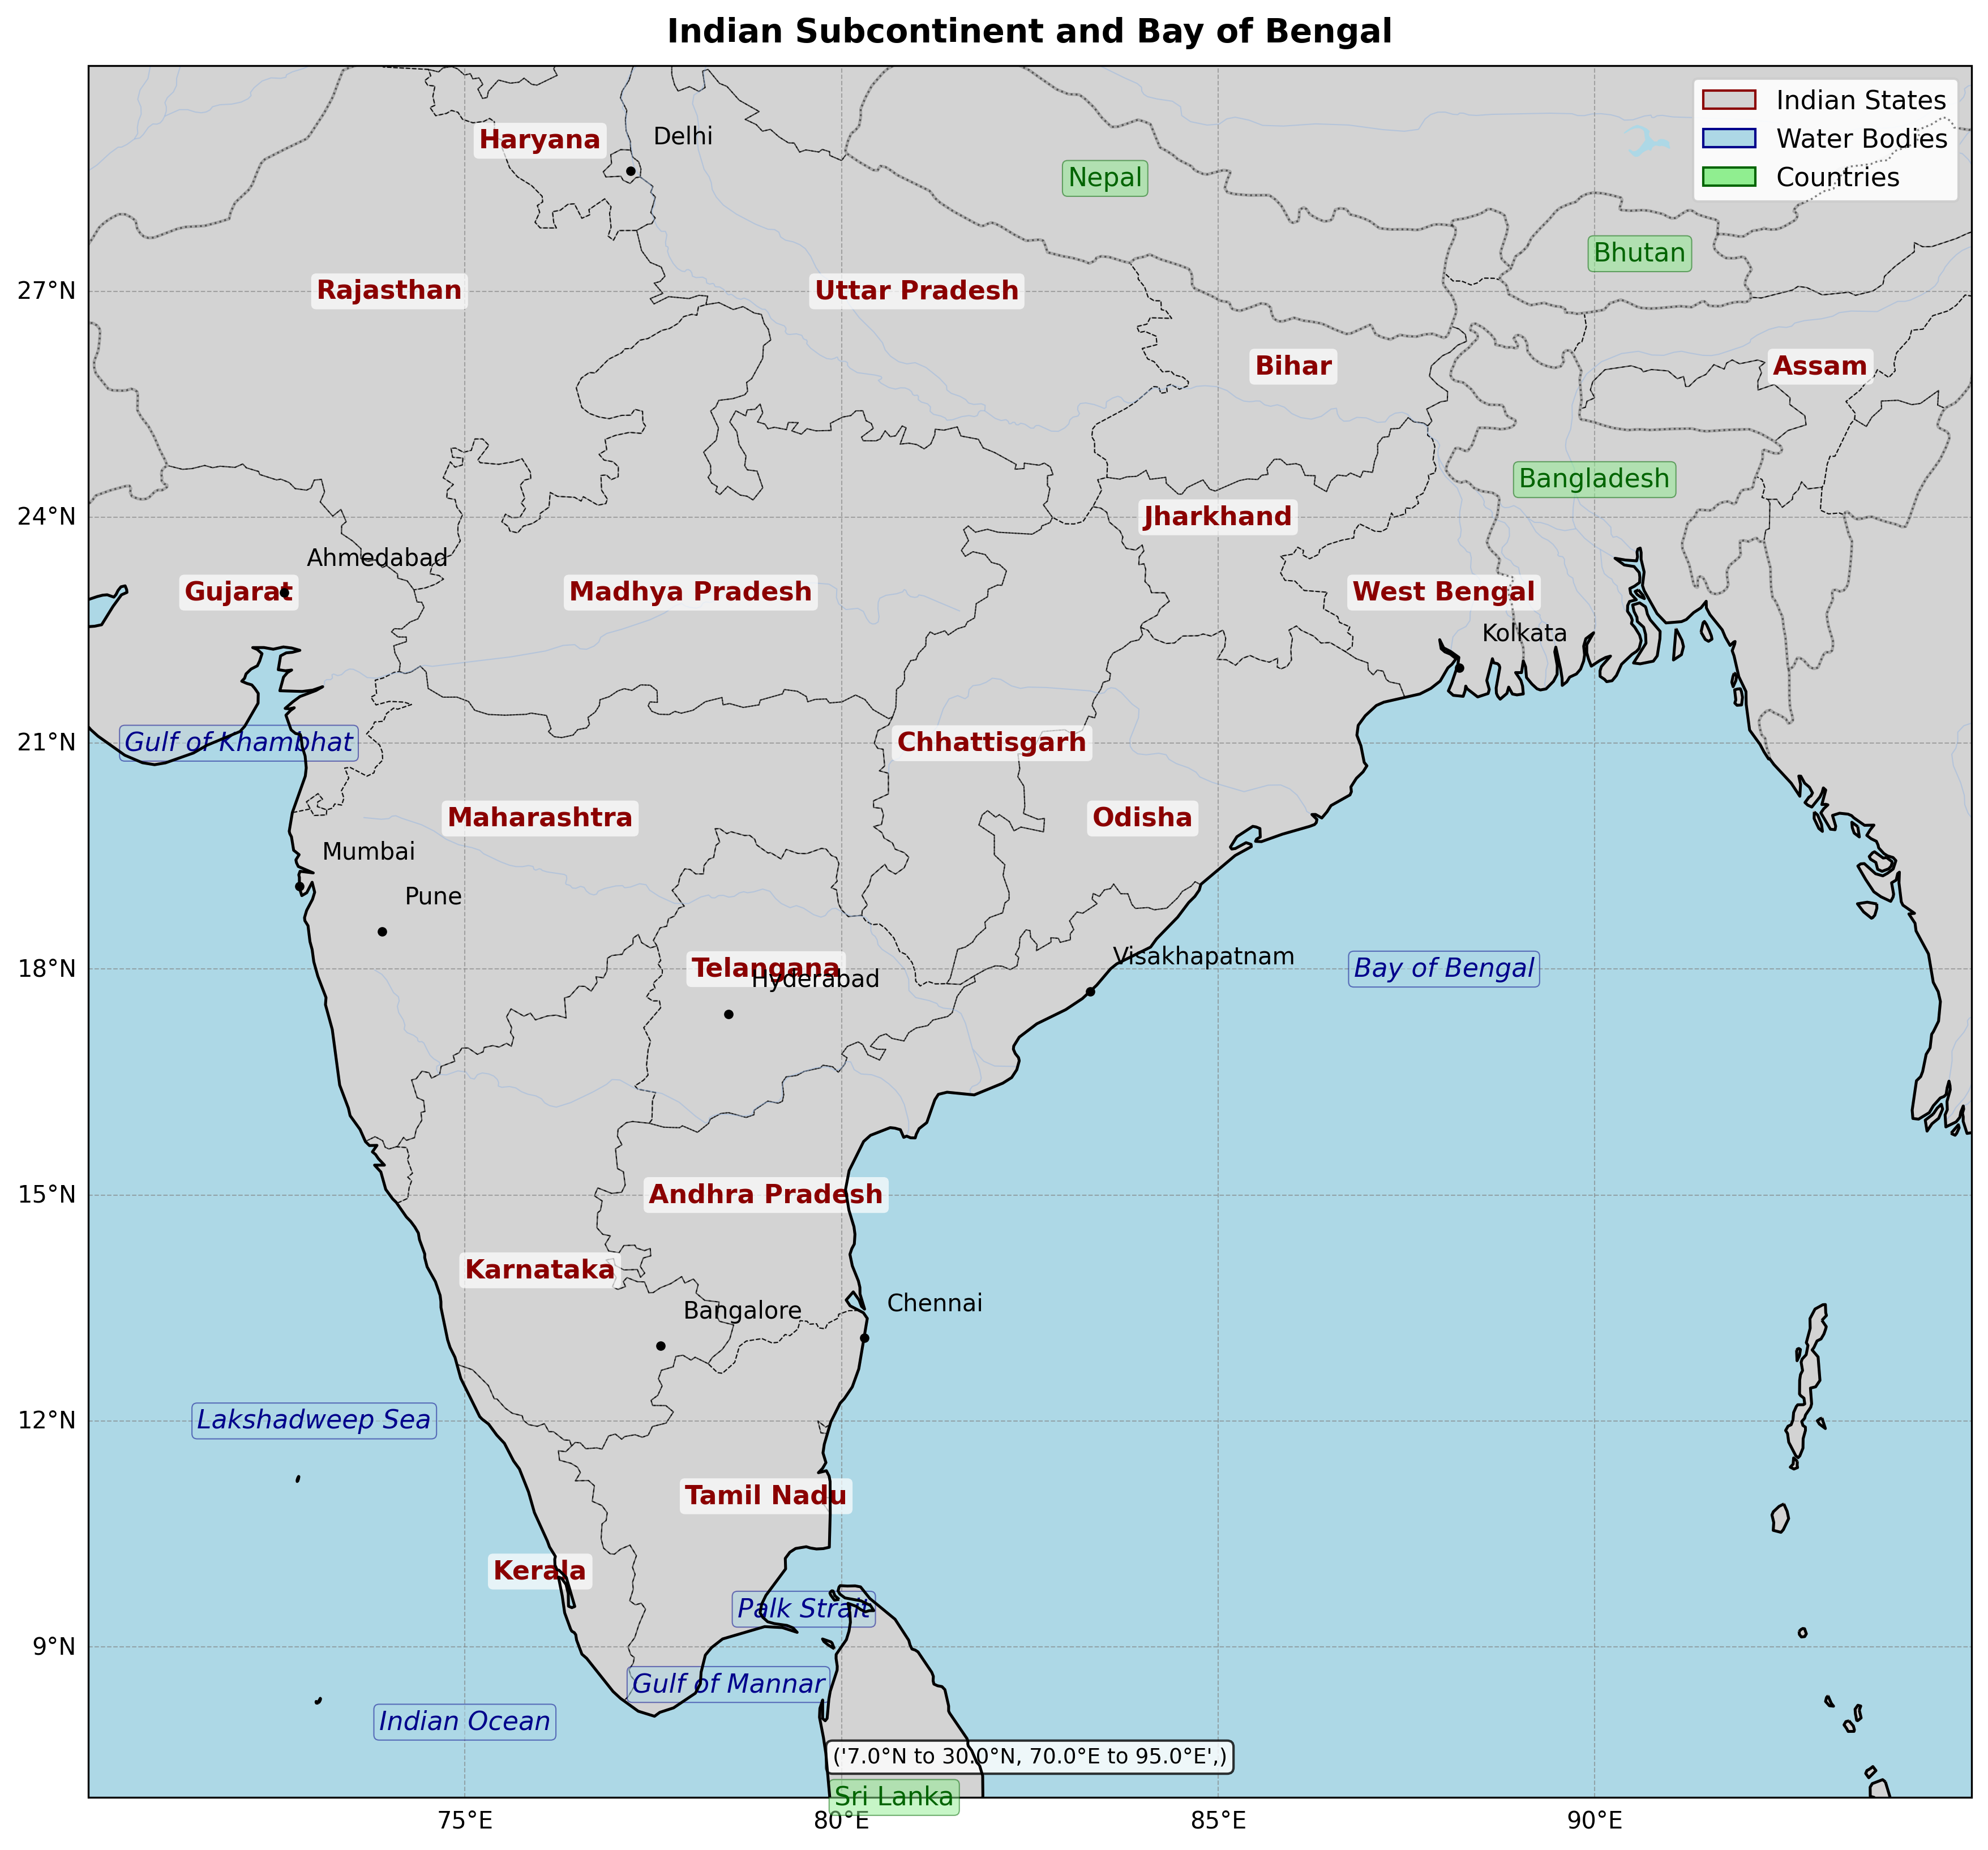
\includegraphics[width=0.87\textwidth]{study_domain_detailed_labels}
  \caption[Study domain region using ERA5 analysis data]{Study domain
  region using ERA5 analysis data (7-30$^\circ$N, 70-95$^\circ$E).}
  \label{fig:study_domain}
\end{figure}

\section{Monsoon Depression Detection and Tracking}
\label{sec:md_detection}

\subsection{Detection Algorithm}
\label{subsec:detection}

MD detection operates on hourly ERA5 850\,hPa relative vorticity using a
threshold-based approach implemented:

\begin{enumerate}
  \item \textbf{Vorticity thresholding}: $\zeta_{850} \geq 4.0 \times
    10^{-5}$\,s$^{-1}$.
  \item \textbf{Local maximum detection}: maxima within a $3^\circ
    \times 3^\circ$ neighbourhood are retained.
  \item \textbf{Closed circulation check}: MSLP within 400\,km radius
    must show a closed cyclonic isobar.
  \item \textbf{Persistence filter}: threshold must be sustained for
    at least 12 consecutive hours.
  \item \textbf{Domain restriction}: track predominantly within
    10-30$^\circ$N, 70-95$^\circ$E.
\end{enumerate}

\subsection{Track Construction and Land-Sea Classification}
\label{subsec:tracking}

Consecutive maxima are linked by nearest-neighbour search with
maximum displacement $5^\circ$ per 6\,h. Land/ocean classification
uses Land-Surface Mask (\texttt{lsm} $\geq 0.5$ for land). Landfall is the first
land-classified point after $\geq 2$ consecutive ocean points.

% %%  FIGURE: Detection algorithm flowchart
% %%  SUGGESTED SOURCE: Draw in draw.io, Inkscape, or using Python's
% % matplotlib patches.
% %%  Show boxes: ERA5 Input -> Vorticity Threshold -> Local Max ->
% % Closed Circ Check
% %%  -> Persistence Filter -> Domain Check -> Track Output -> IMD Validation.
% \begin{figure}[H]
%   \centering
%   %% >> INSERT FIGURE: detection_flowchart.pdf <<
%   %% (Flowchart: ERA5 vorticity -> threshold -> local max -> MSLP check ->
%   %%  persistence filter -> IMD cross-validation -> confirmed MD track)
%   % \includegraphics[width=0.75\textwidth]{detection_flowchart}
%   \caption[MD detection algorithm flowchart]{Flowchart of the ERA5-based MD
%   detection and tracking algorithm.}
%   \label{fig:detection_flowchart}
% \end{figure}

\subsection{IMD Cross Validation and Duration Classification}
\label{subsec:imd_validation}

% ERA5 tracks are matched to annual IMD Monsoon
% records\footnote{\url{https://rsmcnewdelhi.imd.gov.in/report.php}}
% using formation date ($\pm 24$\,h) and landfall location ($\pm
% 2^\circ$). Systems are classified as \emph{short-lived} ($< 96$\,h)
% or \emph{long-lived} ($\geq 96$\,h).

% FIX:
% \section{Rationale for the Azimuthal Hovm\"{o}ller Framework}
\section{Rationale for the Azimuthal Hovm\texorpdfstring{\"{o}}{o}ller Framework}
\label{sec:hovmoller_rationale}

A central methodological challenge in diagnosing land-surface on a
\emph{moving} system is separating the local storm-scale signal from
the background gradient. Fixed-grid analyses of ERA5 latent heat flux
soil moisture India superimpose several confounding signals
simultaneously: seasonal north-south in soil moisture, the spatial
gradient in net heat flux, and large-scale moisture advection. These
signals are spatially coherent and comparable the MD itself, making it
impossible to isolate the storm-induced anomaly.

The Azimuthal Hovm\"{o}ller approach addresses this problem by
re-expressing all in a coordinate system that \emph{follows MD
center}. At each time, the analysis domain is re-centered on the
current track, and all variables expressed as azimuthally averaged
radial profiles relative to the center.

This has three critical advantages:
\begin{enumerate}
  \item \textbf{Background gradient removal.} The radial coordinate
    measures distance from the depression center, not geographic
    position. Systematic north-south or east-west gradients in soil
    moisture or flux therefore appear as uniform offsets in the
    radial coordinate.
  \item \textbf{Time-space coherence.} The Hovm\"{o}ller diagram
    places time (including the critical landfall transition) on one
    axis and radial distance on the other, enabling direct
    before-and-after comparison at every radius simultaneously.
  \item \textbf{Separation of inner-core from outer-band signals.}
    The radial dimension cleanly separates inner-core processes ($r <
    100$\,km, driven by surface energy flux and organised convection)
    from outer-band processes ($r = 100-400$\,km, driven by
    large-scale moisture advection), which is critical for isolating
    the BOE signature.
\end{enumerate}

\subsection{Construction of the Azimuthal Hovm\texorpdfstring{\"{o}}{o}ller}
\label{subsec:hovmoller_construction}

The azimuthal averaging procedure, illustrated in
Figure~\ref{fig:hovmoller_geometry}, is executed at each time step
$t$ relative to the storm center $(\phi_c, \lambda_c)$. Initially, a
radial binning process is applied to all ERA5 grid points within a
400\,km radius of the vortex center. The great-circle distance $r$
for each grid point is determined via the Haversine formula:
\begin{equation}
  r = 2R_E \arcsin\!\sqrt{\sin^2\!\frac{\Delta\phi}{2} +
  \cos\phi_c\cos\phi\,\sin^2\!\frac{\Delta\lambda}{2}},
  \label{eq:haversine}
\end{equation}
where $R_E$ represents the Earth’s mean radius (6371\,km), while
$\Delta\phi$ and $\Delta\lambda$ denote the latitudinal and
longitudinal offsets from the center, respectively. These points are
subsequently partitioned into 16 discrete radial bins of 25\,km
width, spanning $r \in [0, 400)$\,km.

To account for asymmetric features within the storm structure, each
radial bin is further subdivided into 16 equal azimuthal sectors of
$22.5^\circ$. Grid points are assigned to their respective sectors
(ranging from N to NNW) based on their bearing $\theta$ from the storm center:
\begin{equation}
  \theta = \arctan2(\Delta\lambda \cos\phi_c,\; \Delta\phi).
  \label{eq:bearing}
\end{equation}
This discretization divides the storm domain into a polar grid of $16
\times 16 = 256$ sector-annulus segments. Within each segment, the
mean value of the target meteorological variables, such as Latent Heat
Flux (LHF), precipitation, or soil moisture (\texttt{swvl1}), is
calculated by averaging all contained ERA5 grid points.

The final Hovm\"{o}ller representation $H(r, t)$ is assembled by
computing an azimuthal mean of these 16 sector values for each
radius, ensuring equal weighting across the circle. By repeating this
process across the entire temporal domain $t = 1, \ldots, T$, a $16
\times T$ matrix is generated. In the resulting color-filled contour
diagrams (e.g., Figure~\ref{fig:hovmoller_example}), the $x$-axis
represents time-normalized such that $t=0$ marks the landfall
event-and the $y$-axis represents the radial distance from the storm center.

\begin{figure}[ht]
  \centering
  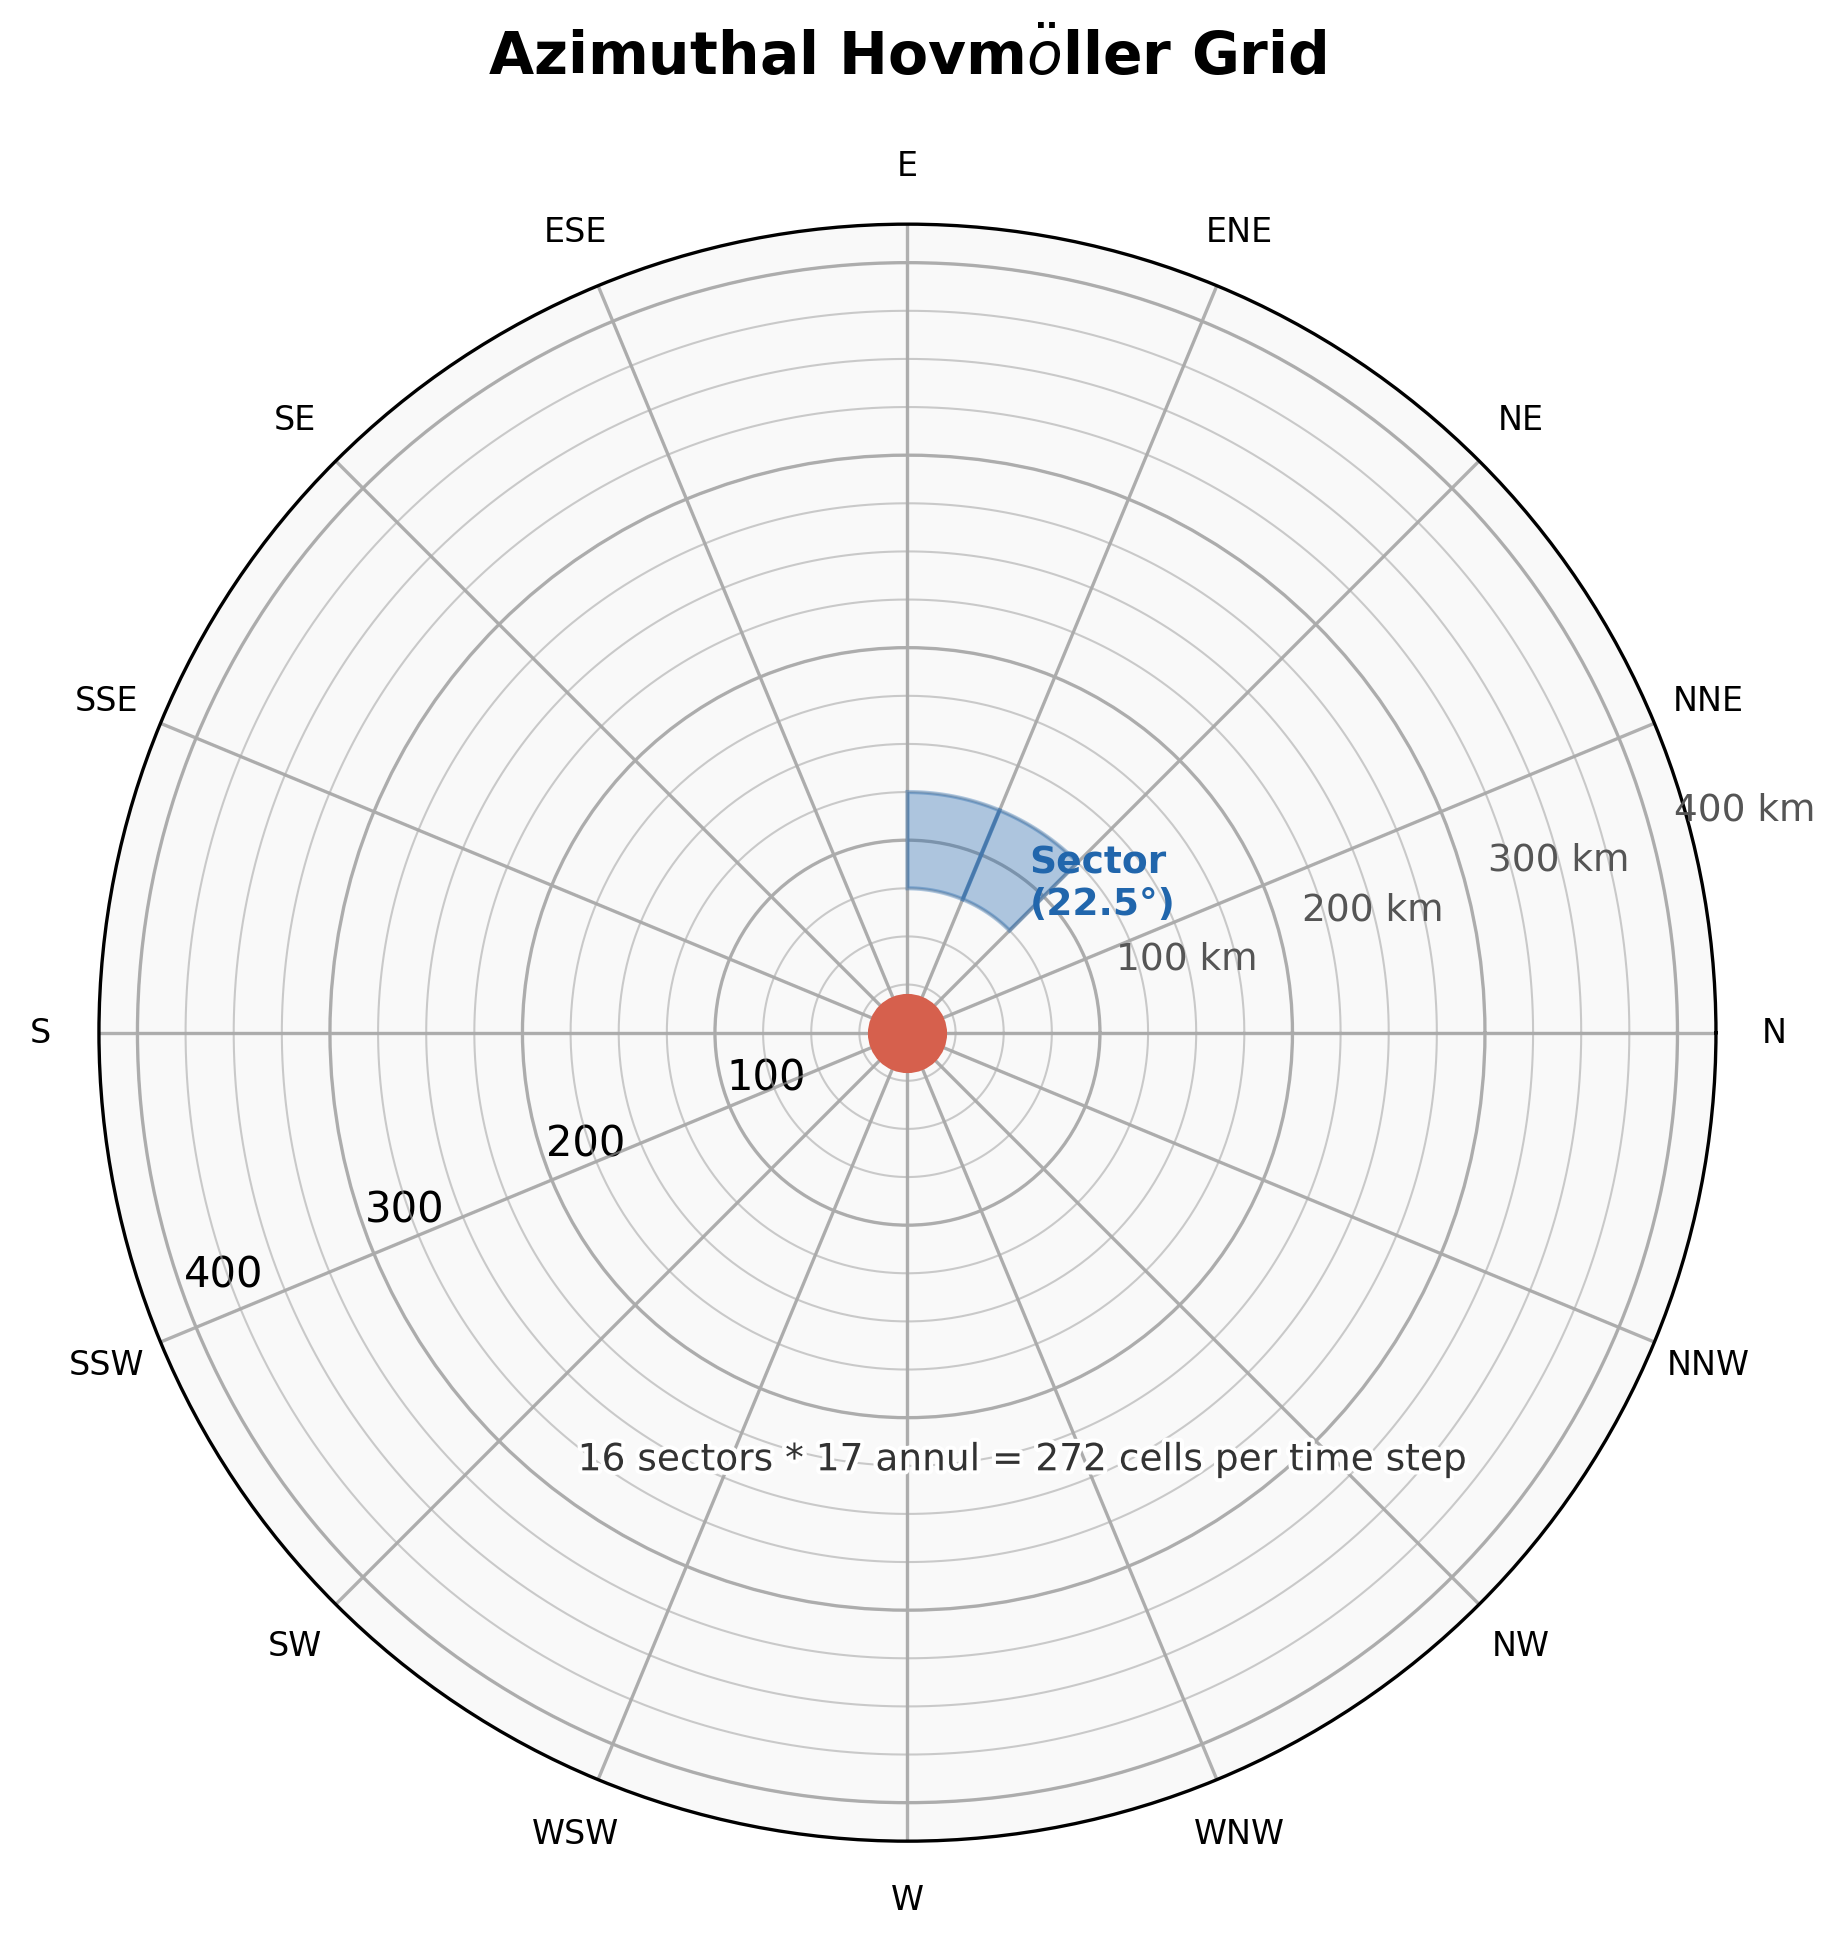
\includegraphics[width=0.65\textwidth]{hovmoller_geometry}
  \caption[Azimuthal Hovm\"{o}ller radial binning geometry]{Polar grid for the
    Azimuthal Hovm\"{o}ller construction. The MD center is surrounded
    by concentric rings at 25\,km intervals to 400\,km, divided into 16
    sectors of 22.5$^\circ$ each. All ERA5 grid points in each
    sector-annulus cell are averaged; the 16 sector values are then
  azimuthally averaged to produce the radial profile at each time step.}
  \label{fig:hovmoller_geometry}
\end{figure}

\subsection{Variables Computed in the Hovm\texorpdfstring{\"{o}}{o}ller Framework}
\label{subsec:hovmoller_variables}

Six variables are computed: total precipitation (mm\,hr$^{-1}$),
surface LHF (W\,m$^{-2}$), surface SHF (W\,m$^{-2}$), near-surface
soil moisture  (m$^3$\,m$^{-3}$), 2-m dew-point
depression ($T_{2m} - T_{d,2m}$, K), and soil tendency
m$^3$\,m$^{-3}$\,hr$^{-1}$.

\section{Diagnostic Framework for BOE Identification}
\label{sec:method_boe_framework}

To distinguish between standard landfall decay and the Brown Ocean
Effect (BOE), this study employs a multi-variate diagnostic framework,
hypothesize that the BOE is not defined by a single variable, but by
the synchronization of mechanical and thermodynamic signals:

\begin{enumerate}
  \item \textbf{Precipitation Structure:} Monitored via azimuthal
    Hovm\"{o}ller plots to identify the transition from broad
    maritime rainbands to a contracted, self-sustaining inner core.
  \item \textbf{Surface Energy Partitioning:} Quantified through
    Latent Heat Flux (LHF) and Sensible Heat Flux (SHF). The BOE is
    characterized by the land surface mimicking the ocean (high LHF, low SHF).
  \item \textbf{Boundary Layer Saturation:} Tracked via 2-m dew point
    ($d2m$) to determine the timescale of continental desiccation and
    the height of the Lifting Condensation Level (LCL).
  \item \textbf{Orography vs. Energetics:} Elevation data from SRTM
    is used to assess if the Eastern Ghats act as a terminal
    mechanical barrier or a thermodynamic trigger for the self-wetting feedback.
\end{enumerate}

\section{Track-Following Time-Series Diagnostics}
\label{sec:timeseries_method}

Track-following time series extract spatially averaged values within
100\,km buffer on the track position at each time step. All time
series are aligned to ($t = 0$). Variables are stratified by
land/ocean classification. Following diagnostic outputs for each confirmed MD:

\begin{itemize}
  \item Time series of surface LHF, SHF, and total heat flux centered on
    landfall, with ocean/land phase shading. Primary plot for BOE
    candidate identification.
  \item Dual-axis time series of \texttt{swvl1} and total precipitation, showing
    co-evolution of surface moisture state and rainfall.
  \item Time series of the Bowen ratio $\beta = Q_H / Q_E$, quantifying the
    land-phase shift in surface energy partitioning.
  \item Equivalent potential temperature $\theta_e$ at the inner-core region
    (0-100\,km), tracking boundary-layer thermodynamic stability.
  \item Dew-point depression computed separately for windward (eastern)
    and leeward (western) sectors of the Eastern Ghats, diagnosing
    boundary-layer moisture asymmetry.
  \item Precipitation recycling ratio $\rho$, quantifying the fraction
    of precipitation sourced from local surface evapotranspiration vs
    large-scale advection.
  \item Diurnal amplitude of the sensible heat flux. A small SHF
    diurnal amplitude indicates a moist surface suppressing daytime
    sensible heating.
\end{itemize}

\begin{figure}[ht]
  \centering
  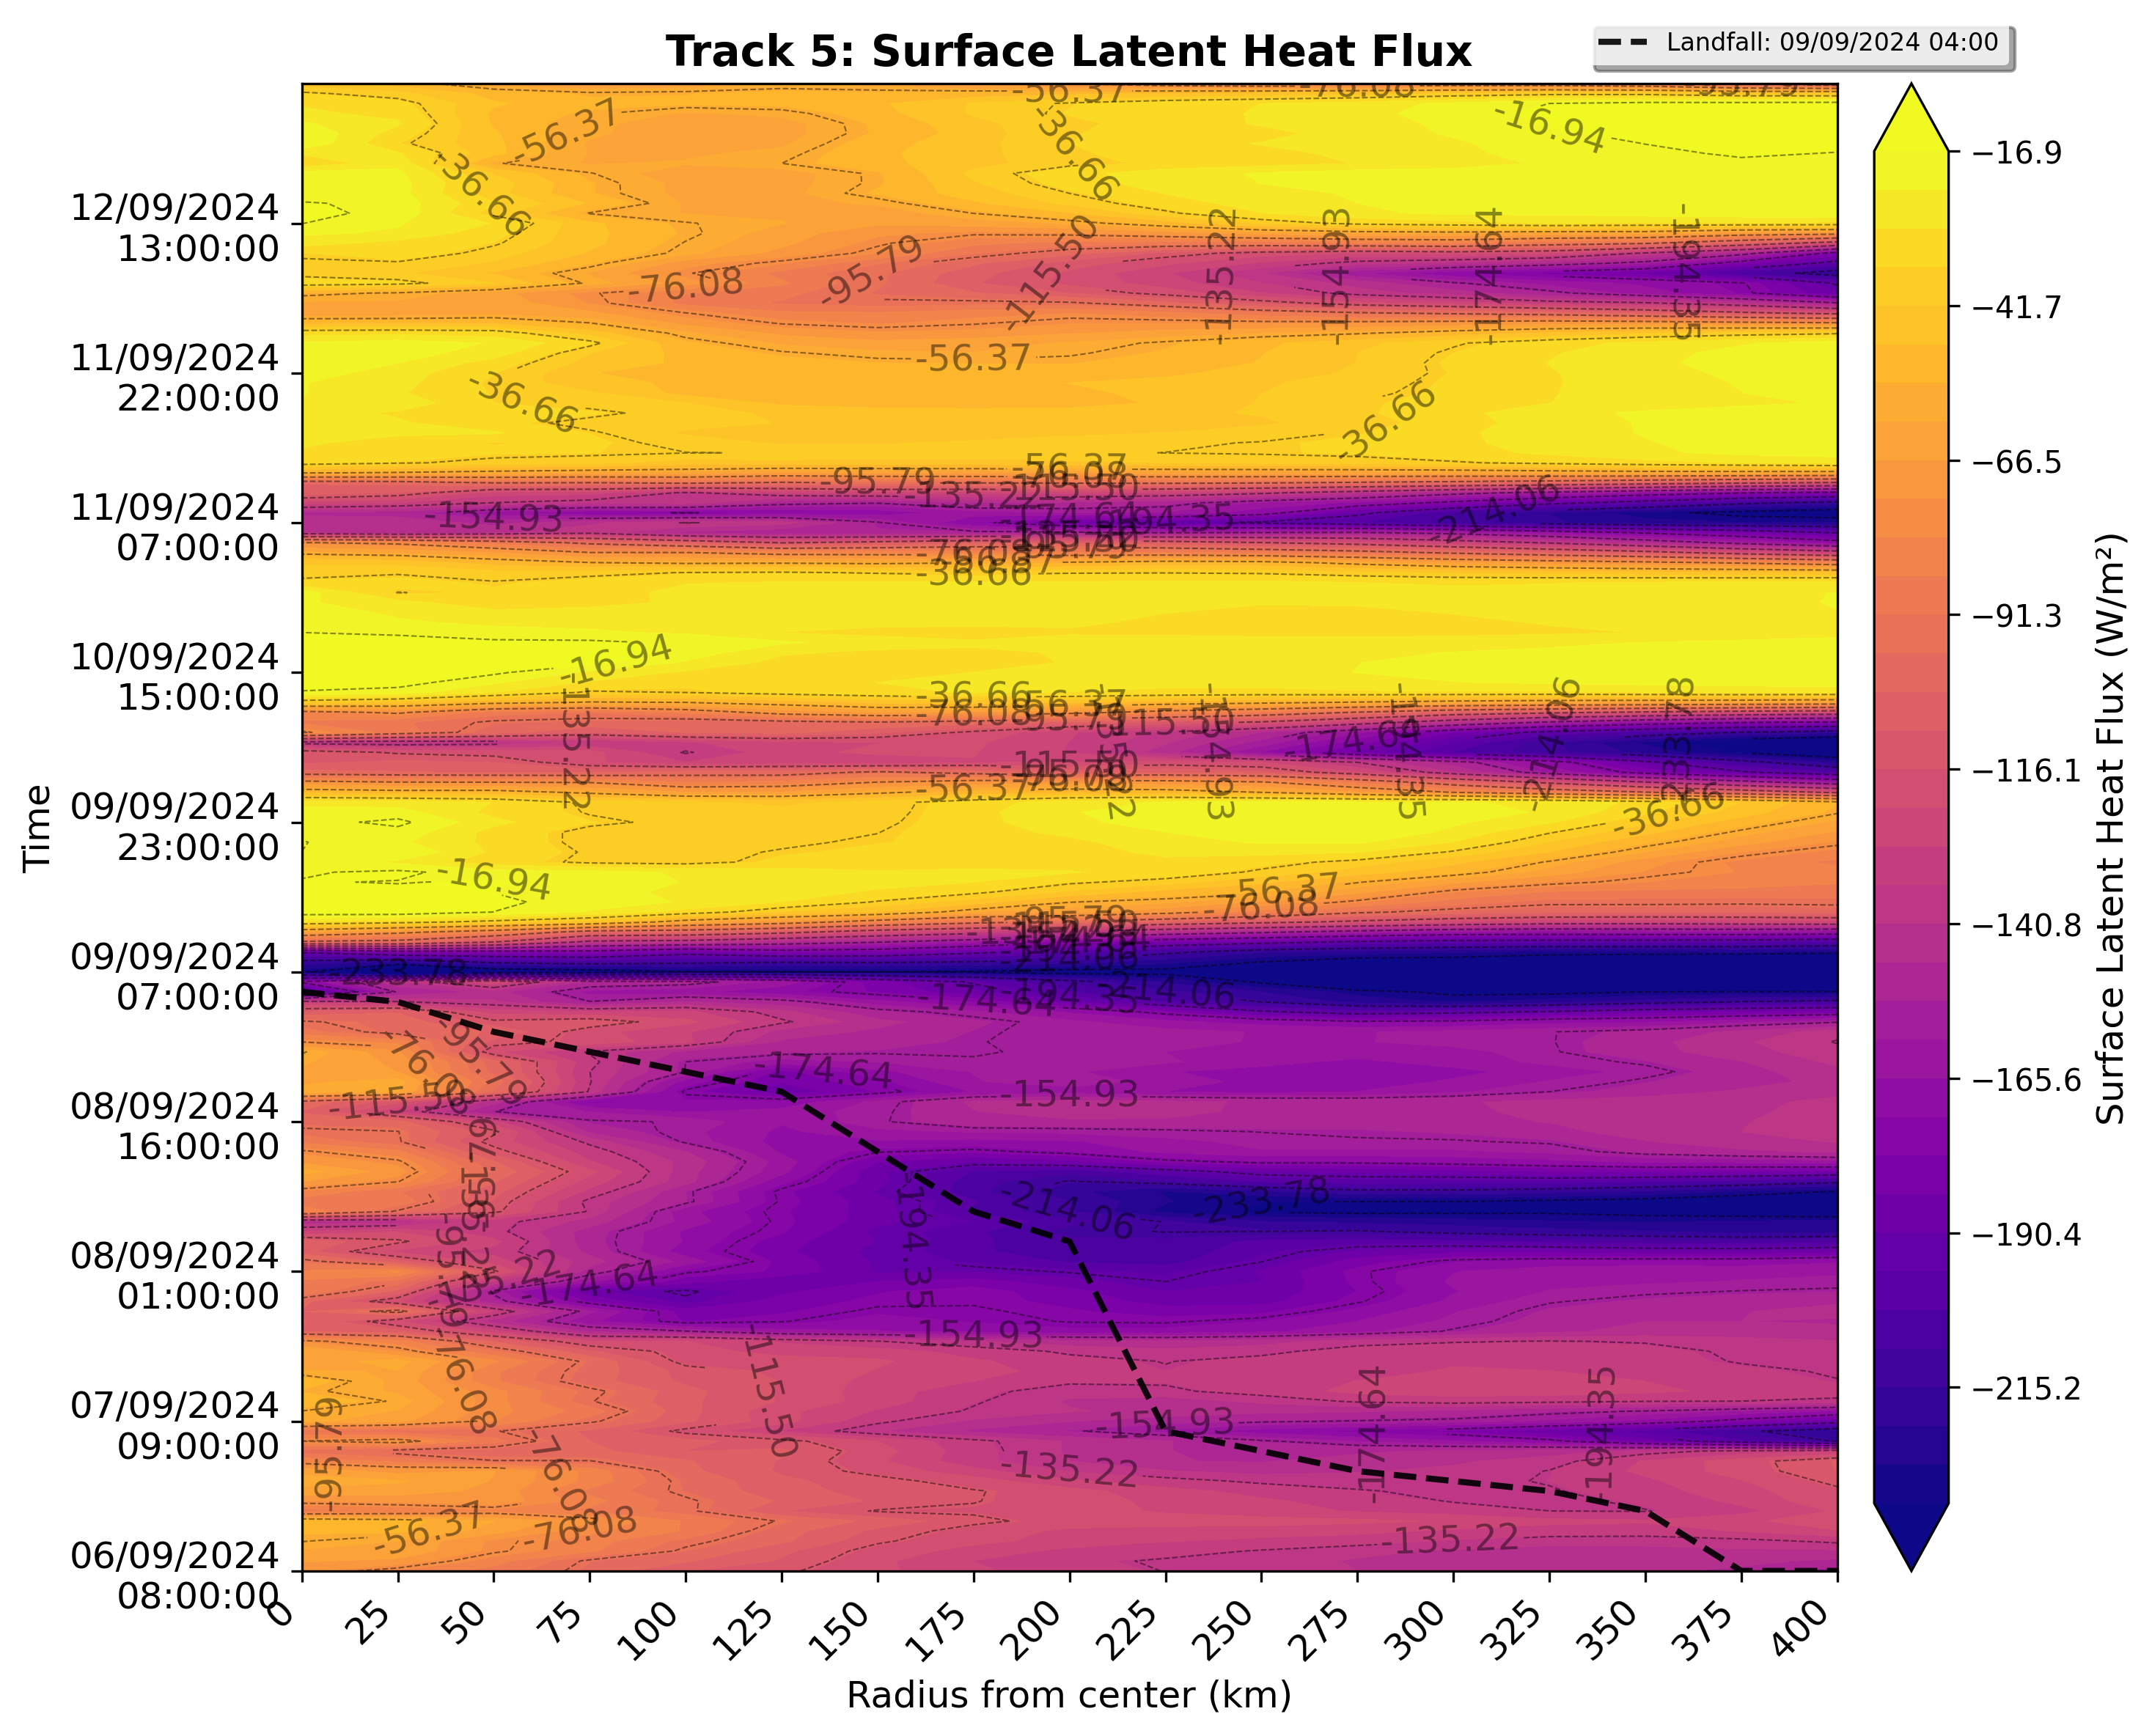
\includegraphics[width=0.8\textwidth]{hov_avg_slhtf_azimuthal_avg}
  \caption[Example annotated Azimuthal Hovm\"{o}ller (LHF)]{Example Azimuthal
    Hovm\"{o}ller of surface LHF (W\,m$^{-2}$) as representative long-lived MD.
    The dashed line marks landfall. Ocean phase and land phase are separated
  at the dashed line.}
  % Inner core ($r < 100$\,km) and outer band ($r = 100-400$\,km)
  % zones are labelled.
  \label{fig:hovmoller_example}
\end{figure}

\section{Surface Heat Flux Analysis and BOE Classification}
\label{sec:heatflux_method}

For each land-falling MD, the 24-hour mean LHF, SHF, and total flux
are computed the windows immediately before and after landfall. A
system is classified as BOE candidate if:
\begin{equation}
  \text{LHF}_\text{land} \geq 70\,\text{W\,m}^{-2}
  \quad \text{for} \geq 18\,\text{consecutive hours.}
  \label{eq:boe_criterion}
\end{equation}

% \section{Antecedent Soil Moisture Index}
% \label{sec:asmi_method}
%
% The ASMI is an exponentially weighted temporal average of
% texttt{swvl1} over the inland track corridor:
% \begin{equation}
%   \text{ASMI}(L) = \frac{\sum_{d=1}^{L} e^{-\kappa(d-1)}\,\bar{S}_d}
%   {\sum_{d=1}^{L} e^{-\kappa(d-1)}},
%   \label{eq:asmi}
% \end{equation}
% with decay constant $\kappa = 0.85$. Lag windows of 24\,h, 3\,d,
% 7\,d, and 14\,d computed. The exponential weighting means that more
% recent soil moisture contribute more than older conditions,
% consistent with the physical that moisture memory decays with time.

% \section{Translational Speed and Terrain Characterisation}
% \label{sec:speed_terrain_method}
%
% Translational speed is computed from consecutive Haversine distances
% by the interval.
% The Terrain Sensitivity Index (TSI) at each track point combines normalised
% elevation contrast ($E^*$), slope ($S^*$), and roughness ($R^*$) from
% the SRTM DEM:
% \begin{equation}
%   \text{TSI} = E^* \times S^* \times R^*.
%   \label{eq:tsi}
% \end{equation}
% A high TSI indicates a complex, steep, rough terrain zone likely to
% decelerate the MD and disrupt its circulation structure.

% \section{Summary of Methodological Workflow}
% \label{sec:method_summary}
%
%%  FIGURE: Methodological workflow
%%  SUGGESTED SOURCE: Draw in draw.io, Lucidchart, or PowerPoint.
%%  Boxes: ERA5 -> MD Detection -> IMD Validation -> Track DB ->
%%  [Hovmoller | Time Series | ASMI | Terrain] -> BOE Classification
% -> Statistics
% \begin{figure}[h]
%   \centering
%   %% >> INSERT FIGURE: method_workflow.pdf <<
%   %% (Flowchart: ERA5 + SRTM inputs -> detection -> four parallel
%   % analysis streams
%   %%  -> BOE classification and statistical output)
%   % \includegraphics[width=0.82\textwidth]{method_workflow}
%   \caption[Overall methodological workflow]{Complete methodological
%     workflow. ERA5 hourly fields feed the MD detection algorithm,
%     producing a validated track database. Each track feeds four parallel
%     analysis streams: Azimuthal Hovm\"{o}ller diagnostics;
%     track-following time-series; antecedent soil moisture index; and
%     terrain characterisation via SRTM. All streams converge in the BOE
%   and statistical analysis stage.}
%   \label{fig:method_workflow}
% \end{figure}
